To validate the iPad application and the features implemented, tests were carried out with various signals applied to the input pins of the Arduino and the signals were received on the app. The signals on the app could then be compared against the actual signals applied to determine qualitatively how well the prototype processed and outputted the signals.



\subsection{Standard Signals}
Firstly, the prototype was tested with standard signals. The voltage applied to each input pin is summarised in Table~\ref{table: standard signals}. The A0 pin on the Arduino, corresponding to the glucose input, was tested with a random noise signal. The A1 pin, corresponding to lactate, was tested with a square wave. The A7 pin, corresponding to potassium, was tested with a sine wave . 

\begin{table}[h!]
\centering
\begin{tabular}{||c c c||} 
 \hline
 Input Pin & Neurochemical & Signal Description \\ [0.5ex] 
 \hline\hline
 A0 & Glucose & Noise signal with 1V P-P voltage, 0.5V offset \\
 A1 & Lactate & 0.1Hz square wave, 1V P-P voltage, 0.5V offset \\
 A7 & Potassium & 0.1Hz sine wave, 0.5V P-P voltage, 0.5V offset \\
 \hline
\end{tabular}
\caption{Standard signals received by input pins}
\label{table: standard signals}
\end{table}

The signals were chosen to have a low frequency of 0.1Hz since the neurochemical signals present during the occurrence of an SD display changes slowly and over a long time frame. Furthermore, the app only receives data once every second from each input, hence according the the Nyquist rate, frequencies above 0.5Hz will undergo aliasing and will not be reconstructed well.

The standard signals inputted to the analogue Arduino pins were produced by a signal generator. In parallel, these signals also went to a PicoScope input channel, which was then connected to a laptop so that the signals could be recorded on PicoLog with a sampling frequency of 5Hz. The signals displayed on PicoLog could then be compared qualitatively with the signals received on the iPad app post processing and transmission. Figure~\ref{fig: test1} shows the set up of the experiment.

\begin{figure}[h!]
\centering
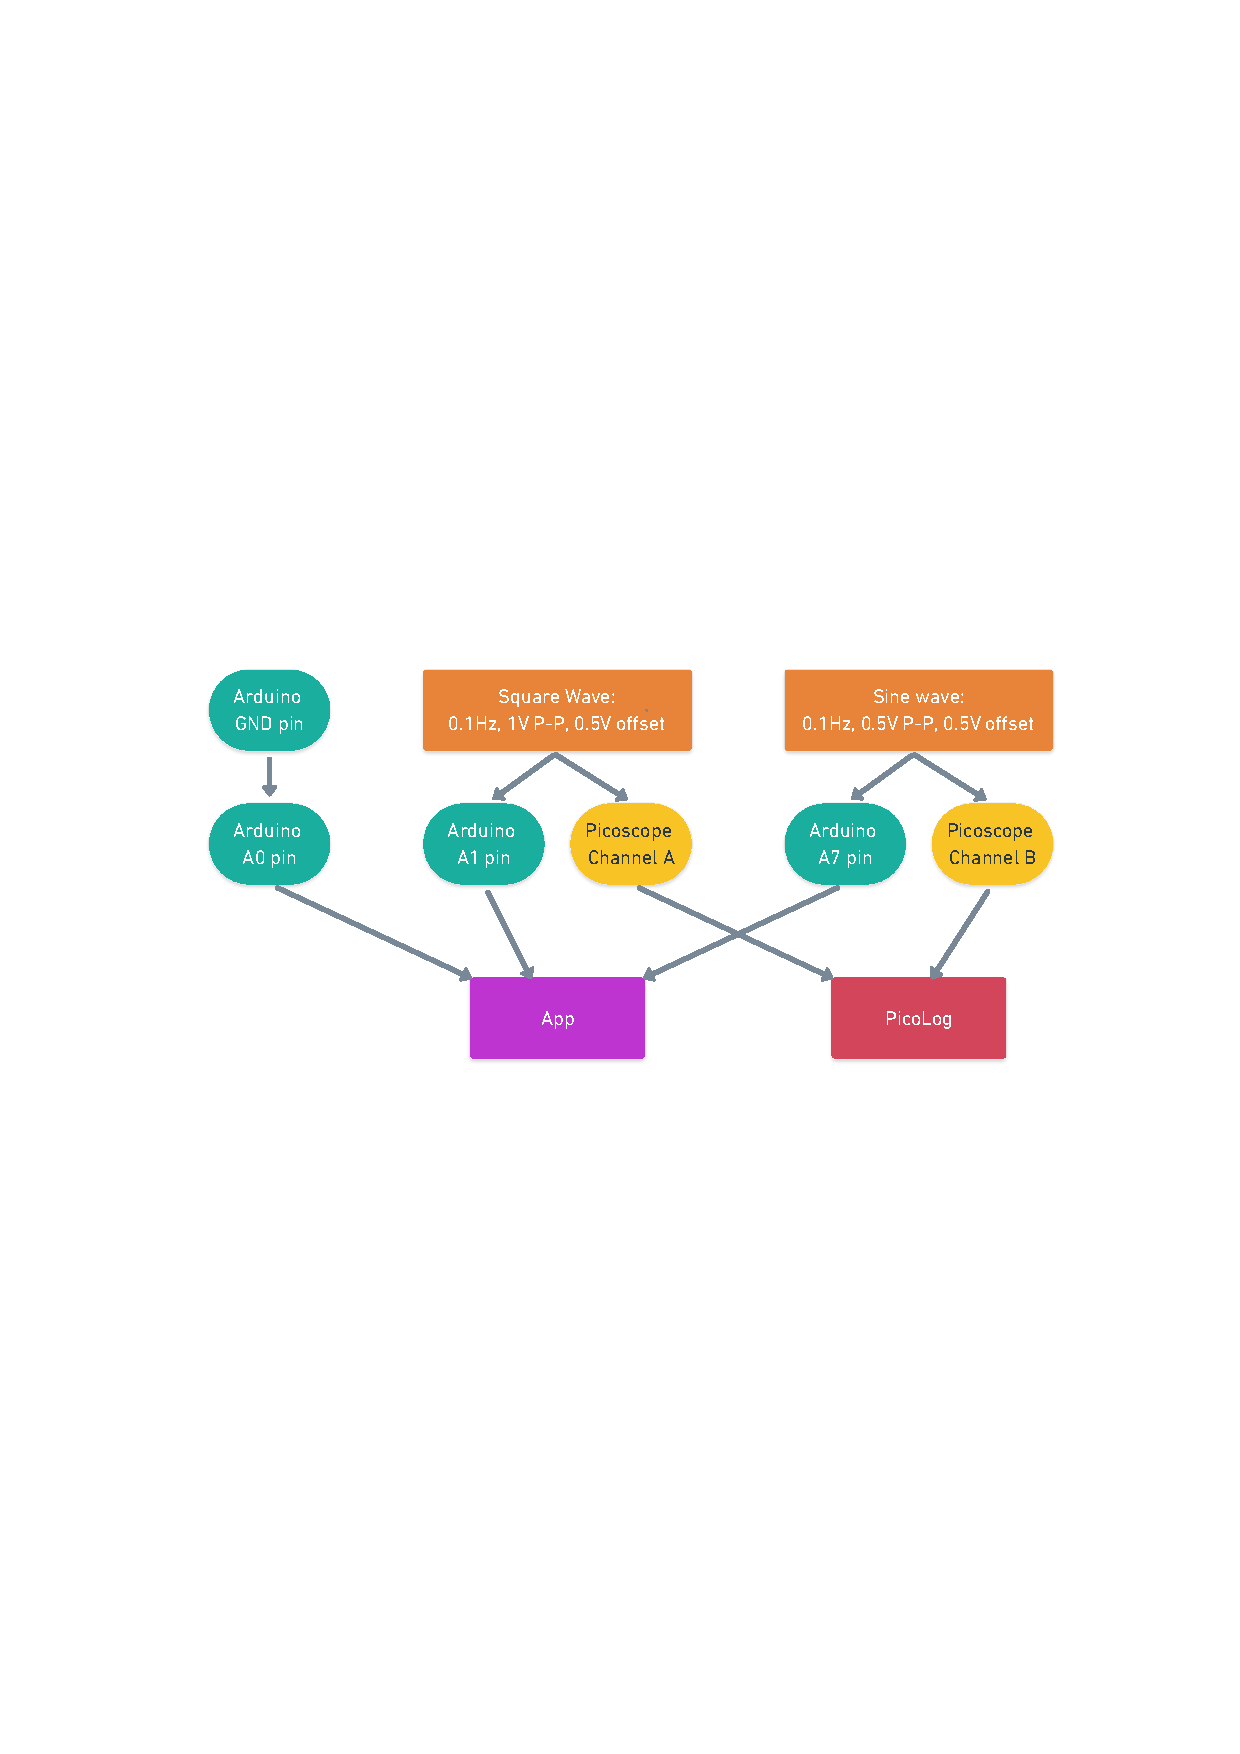
\includegraphics[trim={0cm 0cm 0cm  0cm}, clip, width=.8\textwidth]{./figures/test1.pdf}
\captionsetup{justification=centering}
\caption{Experimental setup for testing standard signals}
\label{fig: test1}
\end{figure}


\subsection{Spreading Depolarisation}